\documentclass[11pt]{beamer}
\usetheme{Madrid}
\usefonttheme{serif}

\usepackage[utf8]{inputenc}
\usepackage[brazil]{babel}
\usepackage[T1]{fontenc}

\usepackage{amsmath}
\usepackage{amsfonts}
\usepackage{amssymb}
\usepackage{graphicx}

\DeclareMathOperator{\sen}{sen}
\DeclareMathOperator{\tg}{tg}

\setbeamertemplate{caption}[numbered]

\author[Rodrigo]{Rodrigo, Thales, Maurício}
\title{Sistemas de Numeração}
% Informe o seu email de contato no comando a seguir
% Por exemplo, alcebiades.col@ufes.br
\newcommand{\email}{email}
%\setbeamercovered{transparent} 
\setbeamertemplate{navigation symbols}{} 
%\logo{} 
\institute[]{Engenharia da Computação \par Organização e Arquitetura de Computadores I} 
\date{} 
%\subject{}

% ---------------------------------------------------------
% Selecione um estilo de referência
\bibliographystyle{apalike}

%\bibliographystyle{abbrv}
%\setbeamertemplate{bibliography item}{\insertbiblabel}
% ---------------------------------------------------------

% ---------------------------------------------------------
% Incluir os slides nos quais as referências foram citadas
%\usepackage[brazilian,hyperpageref]{backref}

%\renewcommand{\backrefpagesname}{Citado na(s) página(s):~}
%\renewcommand{\backref}{}
%\renewcommand*{\backrefalt}[4]{
%	\ifcase #1 %
%		Nenhuma citação no texto.%
%	\or
%		Citado na página #2.%
%	\else
%		Citado #1 vezes nas páginas #2.%
%	\fi}%
% ---------------------------------------------------------

\begin{document}

\begin{frame}
\titlepage
    \begin{figure}[htb]
        \centering
        
\includegraphics[width=0.5\textwidth]{imagens/ufsc.png}
    \end{figure}
\end{frame}

\begin{frame}{Sumário}
\tableofcontents 
\end{frame}

\section{Introdução}

\begin{frame}{Introdução}
    \begin{block}{Gerente}
        Maurício Melo Filho
    \end{block}
    \begin{block}{Front-end}
        Thales Soares de Araújo
    \end{block}
    \begin{block}{Back-end}
        Rodrigo Pontarolo Granemann Melo
    \end{block}
\end{frame}

\begin{frame}{Introdução}
    \begin{center}
        O projeto consiste em uma calculadora de bases que permite a efetuação de distintas operações simultâneamente.
    \end{center}
\end{frame}

\section{Conteúdo}

\begin{frame}{Implementação}
    \begin{center}
        \begin{enumerate}
            \item \textbf{Linguagem de Programação:} \textit{C programming language}
            \item \textbf{Biblioteca Gráfica:} \textit{Ray Library (Raylib)}
            \item \textbf{Coding Style:} \textit{GTK+}
        \end{enumerate}
    \end{center}
    \begin{figure}[htb]
        \centering
        
\includegraphics[width=0.8\textwidth]{imagens/raylib.png}
    \end{figure}
\end{frame}

\begin{frame}{Implementação}
    \begin{block}{Interpretação}
        Uso de analíse léxica e teoria de parsing para realizar recursivamente as operações, respeitado suas respectivas precedências.
    \end{block}

    \begin{figure}[htb]
        \centering
        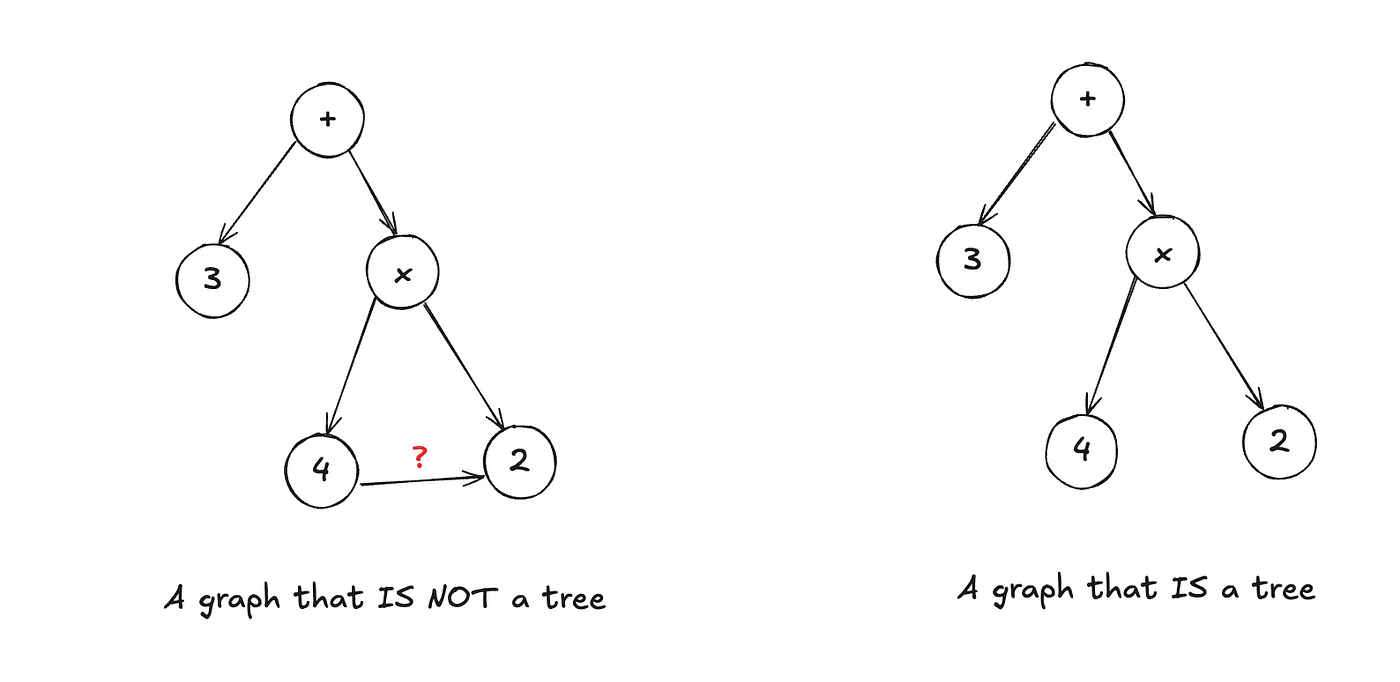
\includegraphics[width=0.8\textwidth]{imagens/graph.png}
    \end{figure}
    
\end{frame}

\begin{frame}{Implementação}
    \begin{block}{Recursão}
        Uso de recursão em prol da legibilidade e redução de código fonte, mantendo a complexidade temporal de $O(n)$.
    \end{block}

    \begin{figure}[htb]
        \centering
        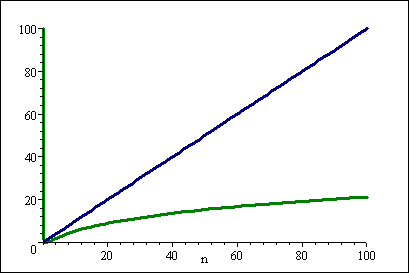
\includegraphics[width=0.6\textwidth]{imagens/time.png}
    \end{figure}
    
\end{frame}

\begin{frame}{Implementação}
    \begin{block}{Graphical User Interface (GUI)}
        Utilizou-se o binding da Ray Library para a linguagem C, que é uma biblioteca primariamente utilizada no desenvolvimento de jogos.
    \end{block}

    \begin{figure}[htb]
        \centering
        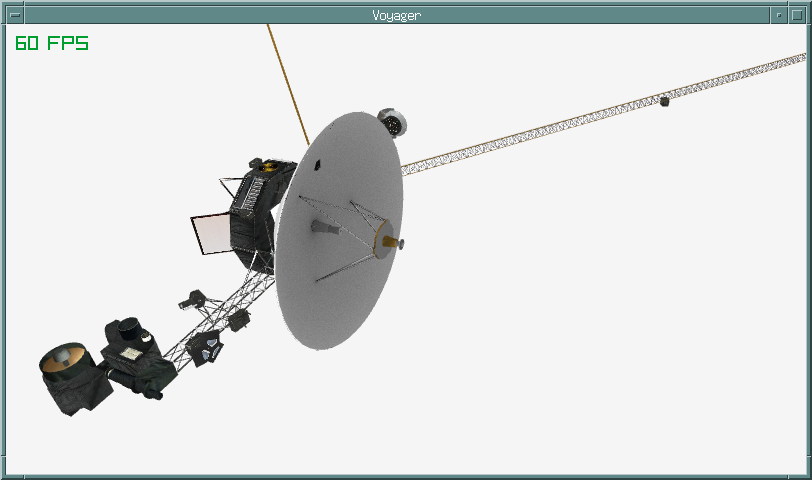
\includegraphics[width=0.8\textwidth]{imagens/rayexample.png}
    \end{figure}
    
\end{frame}

\begin{frame}{Dificuldades}
    \begin{center}
        Não tivemos dificuldades.
    \end{center}
\end{frame}

\begin{frame}{Links}
    \begin{center}
        https://github.com/pontarolo/NumSystem
    \end{center}
\end{frame}

\begin{frame}{Conclusão}
    \begin{center}
        Muito obrigado!
        \begin{figure}[htb]
        \centering
        
\includegraphics[width=0.4\textwidth]{imagens/ufsc.png}
    \end{figure}
    \end{center}
\end{frame}

\end{document}